\documentclass[10pt,twocolumn]{witseiepaper}

% All KJN's macros and goodies (some shameless borrowing from SPL)

\usepackage{KJN}


\usepackage{verbatim} % for writing code in the text
\usepackage{tikz} % for drawing stuff
\usetikzlibrary{positioning} % for relative coordinates
\usepackage{algpseudocode}
\usepackage{algorithm}

\usepackage{listings} %for including code
\usepackage{golang}  % include custom language for Go.
\usepackage{gostyle} % include custom style for Go.
\usepackage{graphicx}
\usepackage{subfig}
\usepackage{color}

\pagestyle{plain}

\addtolength{\oddsidemargin}{-.2in}
\addtolength{\evensidemargin}{-.2in}
\addtolength{\textwidth}{0.4in}

% PDF Info
\ifpdf
\pdfinfo{
/Title  (ELEN4017 Project Report)
/Author (James Allingham and Devin Taylor)
}
\fi

%%%%%%%%%%%%%%%%%%%%%%%%%%%%%%%%%%%%%%%%%%%%%%%%%%%
\begin{document}


\title{Implementation of the HTTP Protocol in Go \\ ELEN4017 Project Report}

\author{James Allingham (672732) and Devin Taylor (603956) - Group 11}
\thanks{School of Electrical \& Information Engineering, University of the
Witwatersrand, Private Bag 3, 2050, Johannesburg, South Africa}



%%%%%%%%%%%%%%%%%%%%%%%%%%%%%%%%%%%%%%%%%%%%%%%%%%%
\abstract{}

\keywords{HTTP, Client-Server, Proxy Server, TCP, UDP, Go programming language}


\maketitle
%\thispagestyle{empty}

%%%%%%%%%%%%%%%%%%%%%%%%%%%%%%%%%%%%%%%%%%%%%%%%%%%%
\section{INTRODUCTION} \label{intro}

Hyper Text Transfer Protocol (HTTP) is a fundamental component of the World Wide Web \cite{kurose}. Understanding HTTP is vital for gaining a well rounded and deep understanding of not only the web and Internet but networking in general. Through understanding HTTP an understanding of protocols as well as the Internet Protocol (IP) networking stack. A collection of web applications, including a client, a server and a proxy server, is to be implemented using a limited subset of HTTP. The goal of this project is to, as closely as possible, match the real world use case for HTTP. The design, implementation and testing of the web application suite is presented in this report along with a critical analysis and recommendations for future improvement of the system. The group work aspects of the project are also discussed. 

%%%%%%%%%%%%%%%%%%%%%%%%%%%%%%%%%%%%%%%%%%%%%%%%%%%%
\section{BACKGROUND}

%%%%%%%%%%%%%%%%%%%%%%%%%%%%%%%%%%%%%%%%%%%%%%%%%%%%
\section{HTTP DESCRIPTION}

The Hyper Text Transfer Protocol has been in existence since 1990 \cite{rfc7230}. It is used by the World Wide Web as an application level protocol for transfer of information in a distributed system. It consists of two programs: a client and a server. The client, also commonly referred to as the browser, communicates with the server by sending it a HTTP request message. The server then responds with a HTTP response message. HTTP is a stateless protocol which means that the server has no knowledge of the client other than the information contained in the request. This is a limitation of HTTP which is overcome with the use of cookies \cite{kurose}. HTTP uses Transmission Control Protocol (TCP) as its underlying transport layer protocol \cite{kurose}. This means that HTTP does not need to worry about reliable data transfer issues such as out of sequence packets or packet loss.  

A typical HTTP communication can be described as follows: 
\begin{enumerate}
	\item A server sets up a TCP listener on one of its ports (an end point for network communication). The default port to HTTP is 80. 
	\item A client initiates a TCP connection with the server (via the server's url) on the appropriate port. 
	\item The client and server complete a `three way handshake' after which each of them have a socket (a virtual data connection between processes) which can be used to send and receive messages. Note that the port associated with these sockets will not be 80.
	\item The client sends a HTTP request message to the server using its socket. This request is received by the server on its matching socket.
	\item The server processes the request and sends an appropriate HTTP response to the client. This communication once again makes use of the sockets that have been set up. 
	\item The server closes the TCP connection.
	\item The client receives the HTTP response before the connection is closed.
\end{enumerate}

	\subsection{Request and Response Messages} \label{formats}

	HTTP is based on communication via request and response messages, both of which have specific formats and can take on a number of values. Both request and response messages contain three parts: the request/ response line, zero or more header lines and an optional body. The format of an HTTP request is shown in \figref{reqformat}. A number of common HTTP request methods are described in \tabref{httpreqs}. The format of an HTTP response is shown in \figref{respformat}. A number of common HTTP response codes are described in \tabref{httpresps}. 2xx responses indicate a success, 3xx responses indicate that client must submit a new request, 4xx responses indicate that the client is in error, and 5xx responses indicate that the server is in error.

	\begin{figure}[htbp]
	\centering
		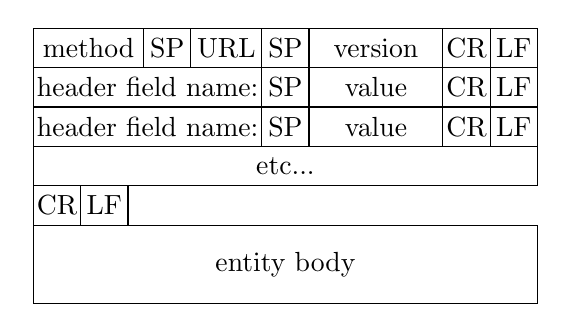
\begin{tikzpicture}
			\draw 
				(0,0) rectangle (1.4,-0.5) node[pos=.5] {method}
				(1.4,0) rectangle (2.0,-0.5) node[pos=.5] {SP}
				(2.0,0) rectangle (2.9,-0.5) node[pos=.5] {URL}
				(2.9,0) rectangle (3.5,-0.5) node[pos=.5] {SP}
				(3.5,0) rectangle (5.2,-0.5) node[pos=.5] {version}
				(5.2,0) rectangle (5.8,-0.5) node[pos=.5] {CR}
				(5.8,0) rectangle (6.4,-0.5) node[pos=.5] {LF}
				(0,-0.5) rectangle (2.9,-1) node[pos=.5] {header field name:}
				(2.9,-0.5) rectangle (3.5,-1) node[pos=.5] {SP}
				(3.5,-0.5) rectangle (5.2,-1) node[pos=.5] {value}
				(5.2,-0.5) rectangle (5.8,-1) node[pos=.5] {CR}
				(5.8,-0.5) rectangle (6.4,-1) node[pos=.5] {LF}
				(0,-1) rectangle (2.9,-1.5) node[pos=.5] {header field name:}
				(2.9,-1) rectangle (3.5,-1.5) node[pos=.5] {SP}
				(3.5,-1) rectangle (5.2,-1.5) node[pos=.5] {value}
				(5.2,-1) rectangle (5.8,-1.5) node[pos=.5] {CR}
				(5.8,-1) rectangle (6.4,-1.5) node[pos=.5] {LF}
				(0,-1.5) rectangle (6.4, -2) node[pos=.5] {etc...}
				(0,-2) rectangle (0.6,-2.5) node[pos=.5] {CR}
				(0.6,-2) rectangle (1.2,-2.5) node[pos=.5] {LF}
				(0,-2.5) rectangle (6.4,-3.5) node[pos=.5] {entity body}
				;
		\end{tikzpicture}
		\caption{HTTP request format}
		\label{reqformat}
	\end{figure}

	\begin{table*}[tb]
		\centering
		\caption{Commonly used HTTP request methods}
		\label{httpreqs}
		\begin{tabular}{p{0.1\textwidth}|p{0.8\textwidth}}
			\hline
			\textbf{Method} & \textbf{Description} \\ \hline
			GET & Request data from the specified URL \\
			HEAD & Request a response identical to the GET response but without the body so that the client can get the header values without retrieving the entire data \\
			POST & Request that the web server accept the data in body, this is often used for filling in forms\\
			PUT & Request that the web server store the data in the body at the specified URL \\
			DELETE & Request that the web server remove the resource stored at the specified URL  \\
			TRACE & Request that the web server echo the request so that the client can detect any changes made to the original request \\
			OPTIONS & Request that the web server inform the client which methods are valid at the specified URL \\
			PATCH & Request that the web server apply a partial change to the resource at the given URL \\
			\hline
		\end{tabular}
	\end{table*}

	\begin{figure}[htbp]
	\centering
		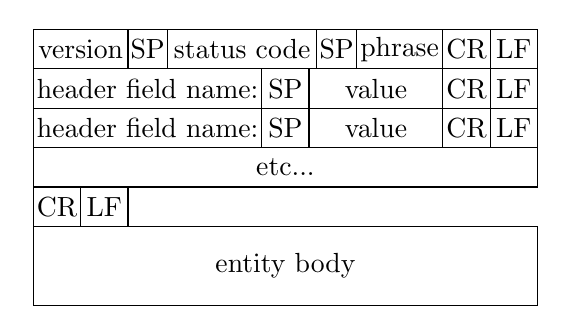
\begin{tikzpicture}
			\draw 
				(0,0) rectangle (1.2,-0.5) node[pos=.5] {version}
				(1.2,0) rectangle (1.7,-0.5) node[pos=.5] {SP}
				(1.7,0) rectangle (3.6,-0.5) node[pos=.5] {status code}
				(3.6,0) rectangle (4.1,-0.5) node[pos=.5] {SP}
				(4.1,0) rectangle (5.2,-0.5) node[pos=.5] {phrase}
				(5.2,0) rectangle (5.8,-0.5) node[pos=.5] {CR}
				(5.8,0) rectangle (6.4,-0.5) node[pos=.5] {LF}
				(0,-0.5) rectangle (2.9,-1) node[pos=.5] {header field name:}
				(2.9,-0.5) rectangle (3.5,-1) node[pos=.5] {SP}
				(3.5,-0.5) rectangle (5.2,-1) node[pos=.5] {value}
				(5.2,-0.5) rectangle (5.8,-1) node[pos=.5] {CR}
				(5.8,-0.5) rectangle (6.4,-1) node[pos=.5] {LF}
				(0,-1) rectangle (2.9,-1.5) node[pos=.5] {header field name:}
				(2.9,-1) rectangle (3.5,-1.5) node[pos=.5] {SP}
				(3.5,-1) rectangle (5.2,-1.5) node[pos=.5] {value}
				(5.2,-1) rectangle (5.8,-1.5) node[pos=.5] {CR}
				(5.8,-1) rectangle (6.4,-1.5) node[pos=.5] {LF}
				(0,-1.5) rectangle (6.4, -2) node[pos=.5] {etc...}
				(0,-2) rectangle (0.6,-2.5) node[pos=.5] {CR}
				(0.6,-2) rectangle (1.2,-2.5) node[pos=.5] {LF}
				(0,-2.5) rectangle (6.4,-3.5) node[pos=.5] {entity body}
				;
		\end{tikzpicture}
		\caption{HTTP request format}
		\label{respformat}
	\end{figure}

	\begin{table*}[tb]
		\centering
		\caption{Commonly used HTTP response methods}
		\label{httpresps}
		\begin{tabular}{p{0.05\textwidth}|p{0.275\textwidth}|p{0.55\textwidth}}
			\hline
			\textbf{Code} & \textbf{Phrase} & \textbf{Meaning} \\ \hline
			200 & OK & HTTP request successful \\
			201 & Created & A new resource was created \\
			202 & Accepted & Request has been accepted for processing \\
			301 & Moved Permanently & The requested resource is now located elsewhere \\
			302 & Found & The requested resource is temporarily located elsewhere \\
			304 & Not Modified & The requested resource has not been modified since last requested - used for caching \\
			400 & Bad Request & The request was not understood by the server \\
			404 & Not Found & The requested resource could not be found \\
			503 & Service Unavailable & The server is temporarily unavailable \\
			505 & HTTP Version Not Supported & The server does not support the HTTP version of the request \\
			\hline
		\end{tabular}
	\end{table*}

	\subsection{Persistent and Non-persistent} \label{pvnp}

	In HTTP version 1.0 (HTTP/1.0), all communication takes the form shown above \cite{rfc1945}. In other words a new TCP connection is made every time the client wants to make a request to the server. However, this approach has its disadvantages. The primary disadvantage is that it is wasteful to repeatedly make new connections when more than one request is going to be made. This is because setting up the TCP connection requires the three way handshake which is a time consuming operation. The solution to this, which was implemented in HTTP version 1.1 (HTTP/1.1), was to allow connections to persist for multiple request-response pairs \cite{rfc7230}. This is accomplished using the \emph{connection} header field, which can take on the values \emph{close} and \emph{keep-alive} for non-persistent and persistent connections respectively.

	\subsection{Proxy Servers and Caching}
	\label{sec:proxy}
	Another limitation of HTTP that results from its statelessness is that it does not have a mechanism for `smart' communication. Consider the following situation:

	\begin{enumerate}
		\item A client requests the file \texttt{Foo.bar}.
		\item The server responds by sending the file to the client by encapsulating it withing an HTTP response message.
		\item The same client receives the file and immediately requests the same file, \texttt{Foo.bar}, again.
		\item The server responds by sending the exact same file to the client again.
	\end{enumerate} 

	The problem with the above situation is that the server is wasting time sending the client the file \texttt{Foo.bar} again because no changes have been made to the file. As a result the server could be slower to respond to other clients. This also increases congestion on the uplink of the Local Area Network of the client. The solution is to make use of a Proxy server (proxy), also known as a web cache. In this situation all HTTP requests are sent to the proxy by default. The proxy then forwards requests to the destination servers. The proxy acting as an intermediary between the clients and server can now store files sent from a server to a client. Now when a client requests the same file in quick succession, the server need only send it once. This solves both problems: the server has a reduced load and the uplink traffic is also reduced. Additionally, because LANs usually have network speeds orders of magnitude larger than the uplink, the client gets the data faster. By making use of the \emph{Last-Modified} and \emph{If-Modified-Since} headers, the proxy can make sure that it always serves the client with the most up to date version of the requested file. This is accomplished with the \emph{Conditional-Get} request. 	

	\subsection{User Datagram Protocol}

	Although HTTP makes use of TCP as it's transport layer protocol, a HTTP-like communication system can be implemented with the User Datagram Protocol (UDP). This would have the disadvantage that it provides unreliable communication. However, it could be faster than if TCP were used.

%%%%%%%%%%%%%%%%%%%%%%%%%%%%%%%%%%%%%%%%%%%%%%%%%%%%
\section{SYSTEM OVERVIEW} \label{sysover}

The system is implemented using HTTP/1.1. This was chosen as it is the most common version of HTTP \cite{}. Some HTTP/1.0 features are still implemented for backwards compatibility and not all HTTP/1.1 features have been implemented.

	\subsection{System Architecture}

	As mentioned, the HTTP protocol follows the Client-Server model. This means that to properly demonstrate the implementation of HTTP, both a client and server are required. Additionally, in order to more extensively represent a real world application of HTTP, a proxy is required. All three of these systems have been implemented in the Go programming language developed by Google. It is a statically typed, imperative, garbage collected, compiled language. It was designed as a system programming language with specific support for networking and multi-threading.

	\subsubsection{Client:}

	The client is responsible for sending HTTP requests to the server. These requests are generated based on user input. This process involves creating the HTTP request in the correct format, as discussed in \secref{formats}, creating a TCP or UDP connection and then sending the request in byte format. The client then waits for a response from the server, decomposing the response into its elements various elements, mentioned in \secref{formats}, and taking an appropriate action based on the response type and contents.

	\subsubsection{Server:}

	The server is responsible for listening for both TCP and UDP connections. Once a connection of either kind is made, the server must handle the client which involves, in the case of TCP, creating a new socket for the communication, and in the case of either TCP or UDP, receiving the HTTP request. The HTTP request must then be decomposed into its elements, discussed in \secref{formats}. Based on the type of request and its contents, the server must take an appropriate action as well as compose and send a HTTP response. Then, in the case of non-persistent TCP connections only, the sever must close the connection.

	\subsubsection{Proxy Server:}

	The proxy is responsible for taking all incoming requests from the client and forwarding them to the destination server. The proxy server must also cache web objects sent, via its self, from the server to the client. This makes use of the \texttt{If-Modified-Since} and \texttt{Last-Modified} header fields to allow the proxy to have the most up to date version of any object in its cache. The proxy acts as both a client and a server in the sense that it is viewed as a server from the perspective of the client and vice versa. As a result it has many of the responsibility listed above.

\subsection{Features}

A number of features were implemented. The ability to use both TCP and UDP was implemented for the client and server. The ability to use both persistent and non-persistent TCP was implemented on the client, server and proxy. Multi-threading was implemented on the server and proxy allowing them to server multiple clients. The ability to track the round-trip-time (RTT) of a message was implemented on the client.

	\subsubsection{TCP vs UDP:}

	This feature allows the user of the client to select the underlying transport layer protocol to use. TCP has the advantage that it offers some robustness in the form of protection against packet loss and delay. On the other hand UDP offers a higher speed than TCP due to its lack of data reliability services. The server implements this feature in terms of the ability to listen for both TCP and UDP connections and handle each appropriately. 

	\subsubsection{Persistent vs Non-persistent:}

	The choice of persistent TCP over non-persistent TCP allows the communication between the client and the server to be sped up for sessions with more than one request. This speed up is a result of not having to perform the three-way handshake every time a request message is sent from the client to the server. This is implemented using the header fields discussed in \secref{pvnp} as well as Multi-threading discussed below in \secref{thread}.

	\subsubsection{Multi-threading:} \label{thread}

	Multi-threading, implemented via \texttt{goroutines}, allows the server (as well as the proxy) to be parallelized. Effectively, this feature allows the server to handle multiple TCP connections at the same time (while also serving clients via UDP connections). This makes the use of persistent TCP feasible as it allows the server to keep listening for new TCP connections even while handling a long persistent communication with the client.

	\subsubsection{RTT timer:}

	This feature allows the client to time how long it takes to receive the response to a message. This could be useful for time out periods or for comparing different types and combinations of communication schemes i.e. TCP vs UDP, persistent vs non-persistent, and proxy vs no proxy.

%%%%%%%%%%%%%%%%%%%%%%%%%%%%%%%%%%%%%%%%%%%%%%%%%%%%
\section{DETAILED IMPLEMENTATION}

HTTP is a large, complex protocol that has evolved over many years. As a result only a subset of the features was implemented in this system. The implemented features will be discussed in detail and important unimplemented features will be mentioned. Additionally the Go language and the implications of implementing the system in this language will be discussed.

	\subsection{Client}

	The client must be capable of dealing with a number of scenarios when making requests to a server. If the server responds with a \texttt{503 Service Unavailable} then the client must resend the request as this is usually a temporary state. On the other hand if the server responds with a \texttt{301 Moved Permanently} or a \texttt{302 Found}, the client must resend the the request to the new location specified by the \texttt{location} header. If neither of those cases are true, then the client must get the header of the response message and using the \texttt{Content-Length} and \texttt{Transfer-Encoding} headers take an appropriate action to ensure that the whole response is received. Following this if the response is a \texttt{200 OK}, the client must search through the HTML for additional objects which must also be requested. This complex process is managed by recursively calling the \texttt{handleRequest} function which takes into account all of the above behaviors. \emph{Algorithm} \ref{handlereq} describes this behavior. Additionally the client must also be aware of whether or not the connection is set to \texttt{keep-alive} or \texttt{close} and keep the connection alive or close it respectively after the message has been received.

	\begin{algorithm}
	\caption{\texttt{handleRequest} Pseudo Code}
	\label{handlereq}
		\begin{algorithmic}
			\State handleRequest(method, url, body, host)
			\State conn $\gets$ Dial(host)
			\State request $\gets$ createRequest(method, url, body, host)
			\State conn.Write(request)
			\State response $\gets$ conn.Read()
			\If{responseMethod $==$ 503}
				\State handleRequest(method, url, body, host)
				\State \Return
			\EndIf
			\If{responseMethod $==$ 301 or 302}
				\State newURl $\gets$ responseLocation
				\State handleRequest(method, newUrl, body, host)
				\State \Return
			\EndIf
			\If {responseTransferEncoding $==$ chunked} 
				\State keep reading until EoF marker
			\ElsIf {responseContentLength $\ge$ bodySize}
				\State keep reading until responseContentLength $==$ bodySize
			\EndIf
			\For{each source in body}
				\State handleRequest(GET, srcURL, , srcHost)
			\EndFor
		\end{algorithmic}
	\end{algorithm}

	The client is missing some important functionality. The most important of which is HTTP Secure (HTTPS), which uses Secure Socket Layer (SSL). A large amount of websites of the Internet now require SSL such as Google and Wikipedia. Without HTTPS the client is unable to access these websites. The main advantage of HTTPS is the improved security and authentication of the visited website which improves privacy and integrity in the exchange of data. This is an increasingly important aspect of Internet communication. This was not added due to time constraints.

	Another important feature that was not implemented was timeout periods. The client does not have a time out period after which it will cease to wait for a response. This means that if the server's response does not reach the client, it will continue to listen for it. This could be easily implemented using the RTT timing code, however, due to time constraints this was not completed.

	\subsection{Server}

	As mentioned the server uses multi-threading to support multiple TCP connections at a time alongside a UDP connection. This is done by creating two threads when the server starts - one for the UDP listener and one for the TCP listener. Each of these then listens for a connection and when one is made it handles the client appropriately. The UDP server communicates with the client in a connectionless manner and as a result can conduct all of the communication on the port used for listening. The TCP server on the other hand uses connections for communication and as a result must create a new port to communicate with the client on. In order to prevent this from locking up with system for long or persistent communication sessions, every time a new client makes a connection, a new thread is created with the purpose of handling the communication on a new port. \texttt{goroutines} are very lightweight which means that they scale well with size and will allow the server to support thousands of simultaneous connections. Note that \texttt{goroutines} are executed concurrently which is not necessarily in parallel. What this means is that although the system will not lock out connections while one is being handled, the system will slow down with too many connections \cite{doxsey}.

	The server accepted the following requests: GET, HEAD, POST, PUT and DELTE. These were considered to be the most important for demonstrating the HTTP protocol. The GET, HEAD and POST methods were the original three methods in HTTP/1.0, while the PUT and DELTE methods provide the missing functionality for the CRUD operations which are very important for many applications which make use of RESTful APIs \cite{guinard}. Other methods that would be useful are those in \tabref{httpreqs}. The PATCH method in particular would be an important addition as it allows much more flexible Update operations by facilitating partial updates of files. This means that when a client wishes to overwrite part of a file they do not need to send the whole file to the server, rather they send only the part they wish to update which saves bandwidth. The OPTIONS method is very useful for allowing clients to query which methods the server accepts. This would reduce the amount of \texttt{400 Bad Request} responses as a result of requests not being understood. These methods were not added due to time constraints. The POST and GET method implemented by the server cannot be used to fill in forms using the \texttt{application/x-www-form-urlencoded} content type. This was not implemented due to time constraints.

	The server is capable of using the following responses: \texttt{505 HTTP Version Not Supported}, \texttt{404 Not Found}, \texttt{400 Bad Request}, \texttt{304 Not Modified}, \texttt{301 Moved Permanently}, and \texttt{200 OK}. These methods cover the majority of common situations. However, some key methods are missing. The \texttt{302 Found} method is useful in real world systems where resources are temporarily moved. Additionally a wider range of 2xx responses are also useful as they give the client more information about the action that has been taken by the server in addition to the fact that their request was successful. Once again, these were not added due to time constraints. The \texttt{403 Forbidden} response would be useful to differentiate between invalid and forbidden requests from the client.

	The server implements a very limited subset of headers. These are: \texttt{Content-Length}, \texttt{Last-Modified}, \texttt{Location}, \texttt{Content-Language}, \texttt{Date} and \texttt{Server}. The \texttt{Content-Length} header is for HTTP/1.0 backwards compatibility. The \texttt{Last-Modified} header, along side the \texttt{304 Not Modified} response, is for use with proxy servers. The \texttt{Location} header is used in conjunction with the \texttt{301 Moved Permanently} response for redirections. The server can also accept a range of headers. Of particular interest here is the \texttt{If-Modified-Since} header which is sent by a proxy to check if it has the most up to date version of a file. An important header that needs to be added is \texttt{Content-Type}, which gives the client important information about the body of the message. 

	Another feature that the server does not support is the use of chunked encoding which allows for data to be streamed. This is particularly useful for dynamically generated content where the length of the content is not known before hand and the \texttt{Content-Length} header cannot be used. Instead the \texttt{Transfer-Encoding} header is used with the value \texttt{chunked}. This lets the client know that they should continue receiving data until the End-Of-File marker is received. This was not implemented because the server does not have any dynamically generated pages and can always use \texttt{Content-Length} as would have been done in HTTP/1.0.

	To facilitate the \texttt{301 Moved Permanently} response, the server maintains a text file that keeps track of moves. When the server receives a request for a URL that does not exist it loads the file into a \texttt{map} data structure and checks if the URL can be found in the \texttt{map}. If it is found, the server returns a \texttt{301 Moved Permanently} response with the location retrieved from the \texttt{map}, otherwise the server returns a \texttt{404 Not Found} response.	

	HTTPS should also be implemented on the server for security reasons. However, HTTPS is fairly complicated as it requires the use of SSL, this is the reason it was not implemented. 

	\subsection{Proxy}

%%%%%%%%%%%%%%%%%%%%%%%%%%%%%%%%%%%%%%%%%%%%%%%%%%%%
\section{DIVISION OF WORK}

	\subsection{Overall Project Management}
	
		The overall project was managed through the use of time management application called Trello. Trello allows job cards to be created and assigned to a member of the group. It has multiple features such as allocating cards as bugs, providing deadlines for cards and allowing for files to be uploaded and shared. All these aspects of the application were used continuously throughout the project. A screen shot of the board that was used for the project can be seen in Figure~\ref{fig:trello} of Appendix~\ref{app:time_man}. \\
		
		The code aspect of the project was managed using git and GitHub. The integration capabilities offered by git meant that the team did not necessarily need to work together all the time, which increased the rate at which work was developed and ultimately lead to the deadline being met. 

	\subsection{Division of Code}
	
		The division of work was such that each member of the group contributed equally to the outcome of the entire project. This was achieved by designating specific subsystems to each member of the group. Devin Taylor was responsible for handling the client code and all associated common functionality, while James Allignham was responsible for handling all the sever code and associated common functionality. From these two bases both engineers contributed equally to the proxy as the majority of the proxy was composed of the subsystems. Table~\ref{tab:functions} in Appendix~\ref{app:other_func}. A screen shot of the GitHub contributions to the project can be seen in Figure~\ref{fig:github} of Appendix~\ref{app:other_func}, this figure emphasises the equal contributions of each engineer. 
	
	\subsection{Division of Report Writing}
	
		The report writing was divided in the same manor as the code, each engineer was responsible for writing about the sections of code that they implemented. The theoretical aspect of the report was divided equally by the aspects that each engineer felt most comfortable contributing to. The introduction, HTTP description, system overview were all done by James Allignham while the results, critical analysis, conclusion and division of work were all done by Devin Taylor.
	

%%%%%%%%%%%%%%%%%%%%%%%%%%%%%%%%%%%%%%%%%%%%%%%%%%%%
\section{RESULTS}

	In order to test the integrity of the system it was necessary to observer the behaviour of the system between two computers over the same network. The primary criteria for testing the system was to ensure the following:

	\begin{itemize}
		\item The client request message was received by the server and interpreted correctly.
		\item The server response message was received by the client, in conjunction with the necessary data, and interpreted correctly.
		\item The client was able to respond to the contents of the servers message by either following a link to the actual site or requesting further information in the form of sources.
		\item The server was capable of returning conditional error codes if necessary.
		\item The client was able to interact with the proxy.
		\item The proxy was able to interact with the client.
		\item The proxy was able to interact with the cache and communicate the corresponding information with the client and server respectively.
	\end{itemize}

	\subsection{Basic Client Server HTTP Requests and Responses} % (fold)
	\label{sub:basic_client_server}
		
		As mentioned in Table~\ref{httpreqs} there are a set of commonly user HTTP requests. For the basis of the project only GET, HEAD, POST, PUT and DELETE were required to be implemented. The use of Wireshark allowed for the message trace between the client and server to be followed. It also provides detailed insight into the communications by being able to analyse the messages being sent and received. For all the examples provided below assume that the client IP address is 10.0.0.148 and the server IP address is 10.0.0.243. These IP addresses will provide insight into the trace observed between client and server when they communicate.
		
		\subsubsection*{The GET and HEAD Methods:} With reference to Figure~\ref{fig:basic_get} of Appendix~\ref{sub:wireshark_results} the client sends a GET request to the server, to which the server responds with an OK message containing the contents of the file that was requested. The OK message symbolises that the server was able to access the requested file. The second GET message sent for \texttt{/test.jpg} is due to the fact that the returned file contained an image and as a result the client is able to detect the presence of sources and request them from the applicable server. In this example the image was hosted on the same server. \\
		
		An example of the GET message sent can be seen in Figure~\ref{fig:basic_get_message} of Appendix~\ref{sub:wireshark_results}. The aspects of interest are the inclusion of the required URI in headers as well as the method (GET) in the request line. This is contrary to what is observed in Figure~\ref{fig:basic_get_response} of Appendix~\ref{sub:wireshark_results} whereby there is no mention of a URI but there is the inclusion of the \texttt{Data} section, symbolising the entity body, which contains the requested content. These two figures highlight the fundamental differences between the HTTP messages sent by the client and the HTTP messages sent by the server. \\
		
		Fundamentally the communication between the client and the server for the HEAD request is the same as the GET request. The only difference observed is that the response message from the server contains no entity body (\texttt{Data} section) but rather only the header information. 
		
%		\subsubsection*{The HEAD Method:} 
		
		\subsubsection*{The POST and PUT Methods:} The post method differs from the above mentioned methods in the sense that the client includes an entity body in the request message sent to the server. As mentioned in Table~\ref{httpreqs} the POST method is commonly used for interacting with forms, hence the body that's included in the client request message contains the information that needs to be submitted to the form. An example of the trace between the client and the server takes on the same form as mentioned above, this can be seen in Figure~\ref{fig:basic_post} of Appendix~\ref{sub:wireshark_results}.
		
%		\subsubsection{The PUT Method:}
		 The PUT method has the same face value structure as the POST method with regards to the trace observed between the client and server. The two methods only differ in how the client handles the requested URI as well as the entity body included in the client's request message. These differences are detailed in Table~\ref{httpreqs}.
		 
		 \subsubsection*{The DELETE Method:} The DELETE method also has the same trace structure as the above mentioned methods, see Figure~\ref{fig:basic_delete} of Appendix~\ref{sub:wireshark_results}, whereby the client makes a request and the server responds to the request. The difference with the DELETE method is that the URI included in the request message links to the file on the server that the client wishes to remove. The server subsequently responds to the client whether or not it was able to remove the file. 
	 
	 \subsection{Client Server HTTP Requests and Responses Via Proxy}	
	 
		 The communication observed between the client and server, via the proxy, follows the same basic structure in the sense that a request message is sent by the client and a response message is received back. The communication differs in the sense that the proxy acts as an intermediary relaying the message from the client to the server and the server to the client. The details pertaining to how this is accomplished are detailed in Section~\ref{sec:proxy}. A test was conducted on three different computers on the same network in order to recreate the trace sequence observed with a proxy being used. The client was represented on \texttt{192.168.1.103}, the proxy on \texttt{192.168.1.104} and the server of \texttt{192.168.1.105}. \\
		 
		 The trace sequence observed for a GET message can be seen if Figure~\ref{fig:proxy_new} of Appendix~\ref{sub:wireshark_results}. An initial GET request was sent by the client to the proxy for the \texttt{/index.html} file. The message sent to the proxy can be seen in Figure~\ref{fig:proxy_new_client} of Appendix~\ref{sub:wireshark_results}, the important aspect of this message to note is the inclusion of the servers IP address under the host heading. Once the proxy receives the request it checks if the requested file was saved in its cache, which it was not, and forwarded the request to server. The server then retrieves the requested file, which is passed by to the client via the proxy. The response from the server contains an \texttt{Last-Modified} header line which is fundamental for the caching of the proxy, this can be seen in Figure~\ref{fig:proxy_server} of Appendix~\ref{sub:wireshark_results}. \\
		 
		 The above experiment was repeated again expect this time the proxy has added the \texttt{/index.html} file into its cache. The trace sequence can be observed in Figure~\ref{fig:proxy_cache} of Appendix~\ref{sub:wireshark_results}. It can be noted that the sequence is the same as described above except the response code from the server is a \texttt{304 Not Modified}. This occurs because the proxy registered that the requested \texttt{/index.html} file was in its cache and forwarded an \texttt{If-Modified-Since} header line in its request to the server, this date corresponds to the date returned from the server in the previous example. A comparison between the proxy GET request before and after caching can be seen in Figure~\ref{fig:proxy_comparrison} of Appendix~\ref{sub:wireshark_results}. Due to the \texttt{304} response from the server the proxy then retrieves the requested file from its cache and forwards a copy of this to the client.
	
	\subsection{Server Error Codes}
	
		Additional tests were also conducted between the client and server to ensure that all the server error codes were implemented correctly. The specific errors that were implemented were provoked as follows:
		
		\begin{table}[htbp]
			\centering
			\caption{Different methods for invoking server response errors}
			\label{tab:errors_responses}
			\begin{tabular}{p{0.3\columnwidth}| p{0.6\columnwidth}}
				\hline
				\textbf{Status Code} & \textbf{Provocation}\\ \hline
				301 & Request a file that had been moved to a new location on the local server \\
				400 & Make a request that did not fall within the range of accepted/implemented requests \\
				404 & Request a file that did not exist on the server \\
				505 & Alter the HTTP version used in the request message \\
				\hline
			\end{tabular}
		\end{table}
		
		The corresponding server responses can be seen in the trace sequences in Figure~\ref{fig:server_error} of Appendix~\ref{app:rtt}. It can be noted that the \texttt{301} response message invoked a new request to be generated by the client to the location that the file had been moved to. The client is able to make the new request as a result of the \texttt{Location} header line returned by the server in the header field, this can be seen in Figure~\ref{fig:301} of Appendix~\ref{app:rtt}.
	
	\subsection{Round Trip Time Calculations}
	
		A timer class was created in order to determine the Round Trip Times (RTT) observed for different settings on the system. The different systems settings are detailed in Section~\textcolor{red}{NEED A SECTION REFERENCE FOR THIS}. \\
		
		The results obtained from these calculations were written to a text file and plotted using a graphing library, the results can be seen in Figure~\ref{fig:rtt}. The tests were conducted on retrieving the same \texttt{/index.html} for each situation. The results obtained are as expected, whereby the fastest time was TCP with a persistent connection and no proxy while the slowest time was a TCP non-persistent connection going through the proxy. 
		
		\begin{figure}[htbp]
			\centering
			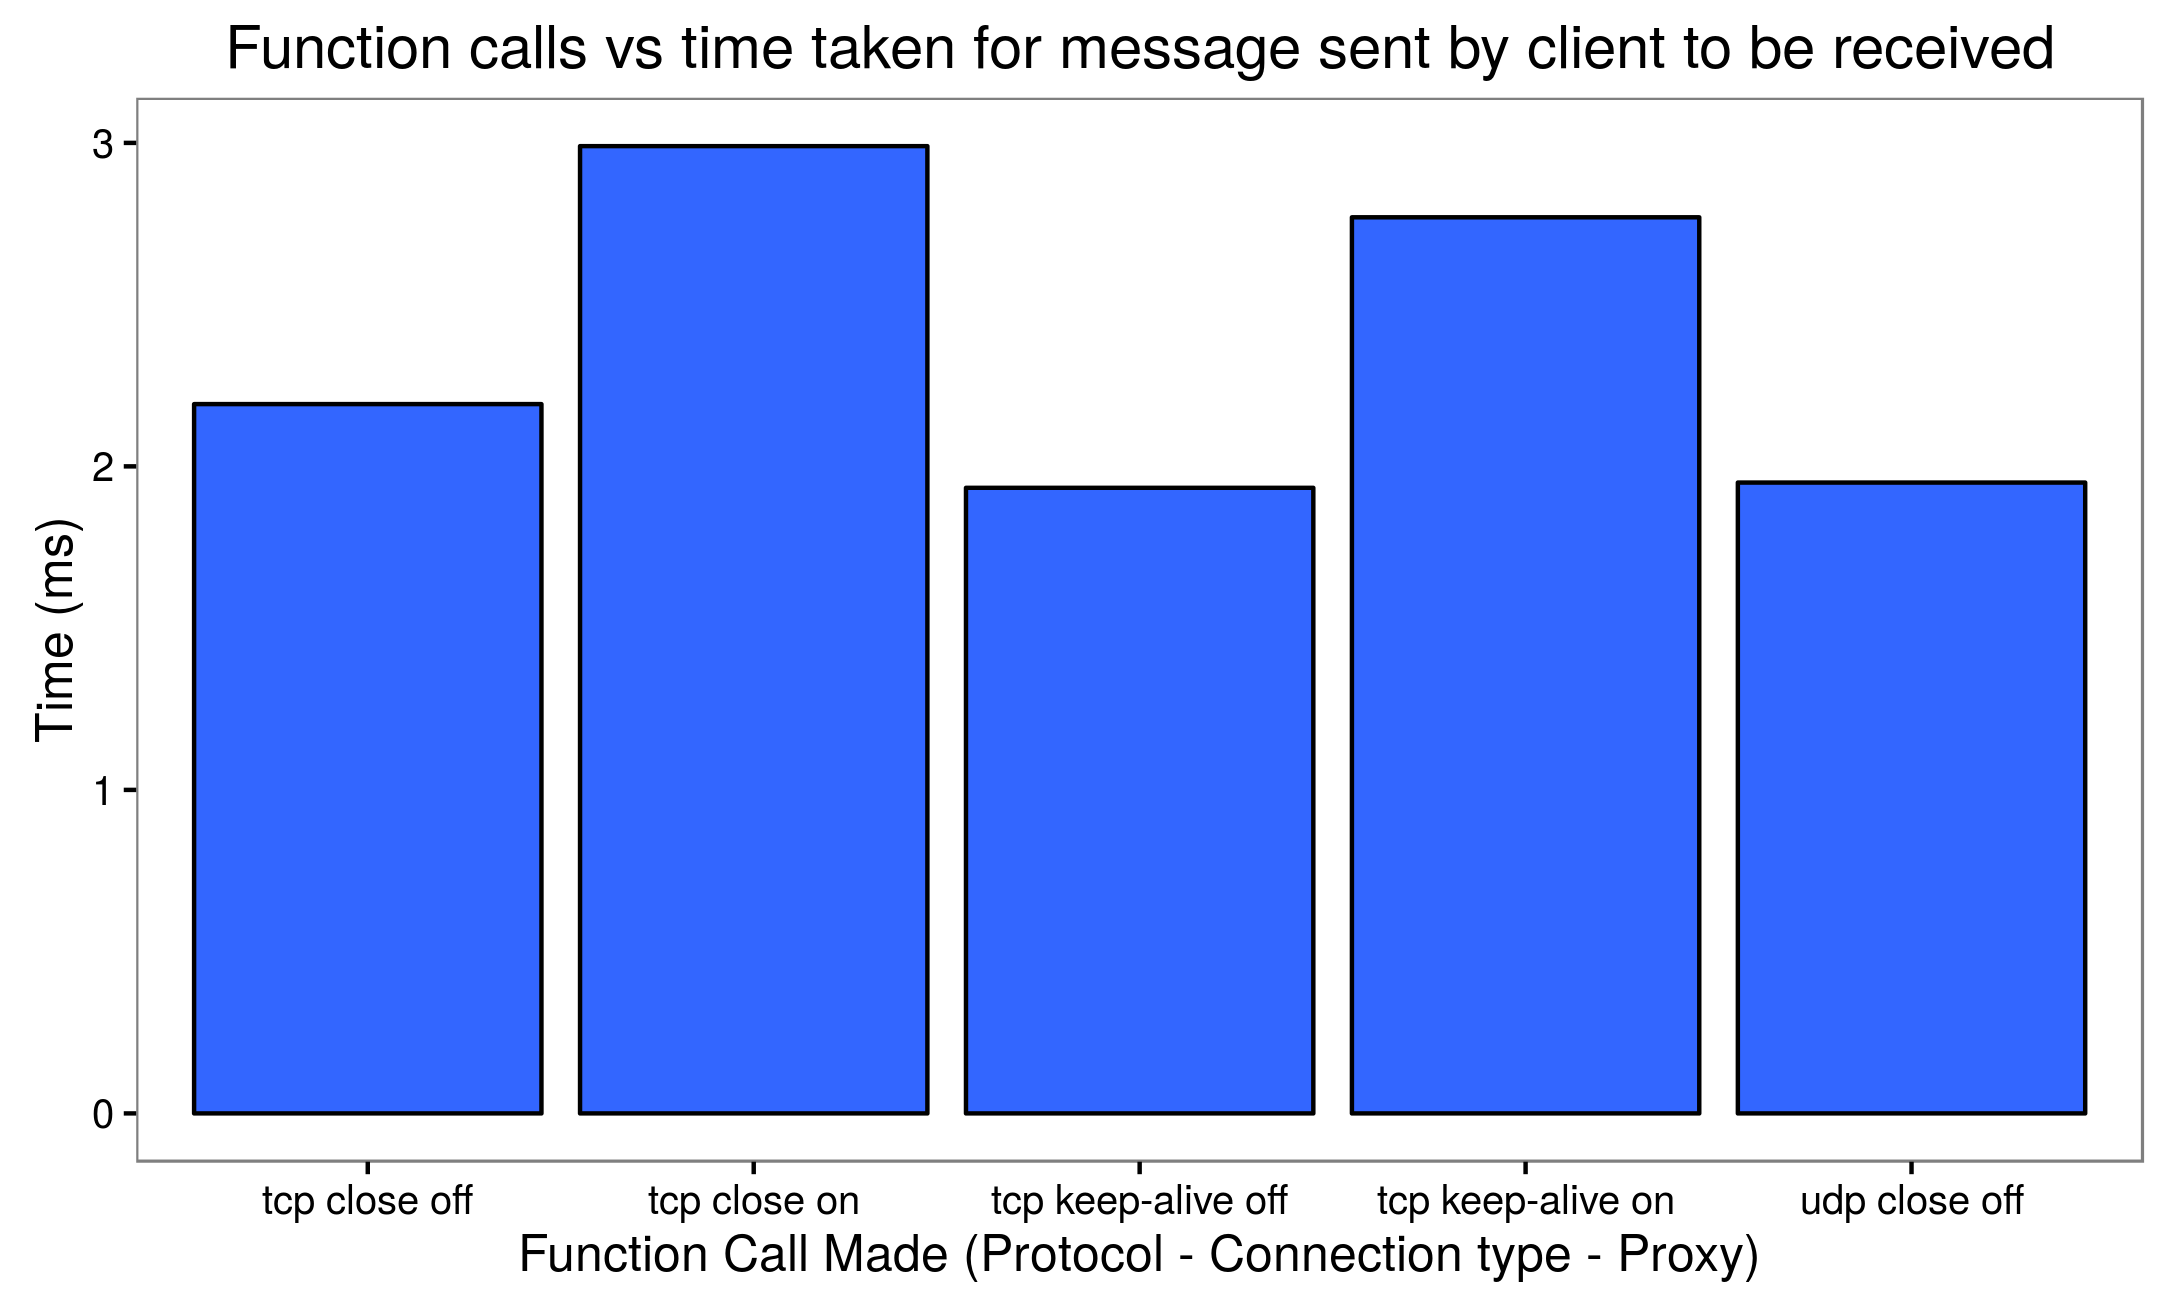
\includegraphics[width=\columnwidth]{resources/RTT.png}
			\caption{RTT times for different connection type settings}
			\label{fig:rtt}
		\end{figure}
		
		The same experiment was conducted to determine the effectiveness of the cache on the rate at which the information is retrieved by the client. The results can be seen in Figure~\ref{fig:rtt_cache}, it can be noted that the once the \texttt{/index.html} file had been cached the client was able to retrieve the information faster.
		
		\begin{figure}[htbp]
			\centering
			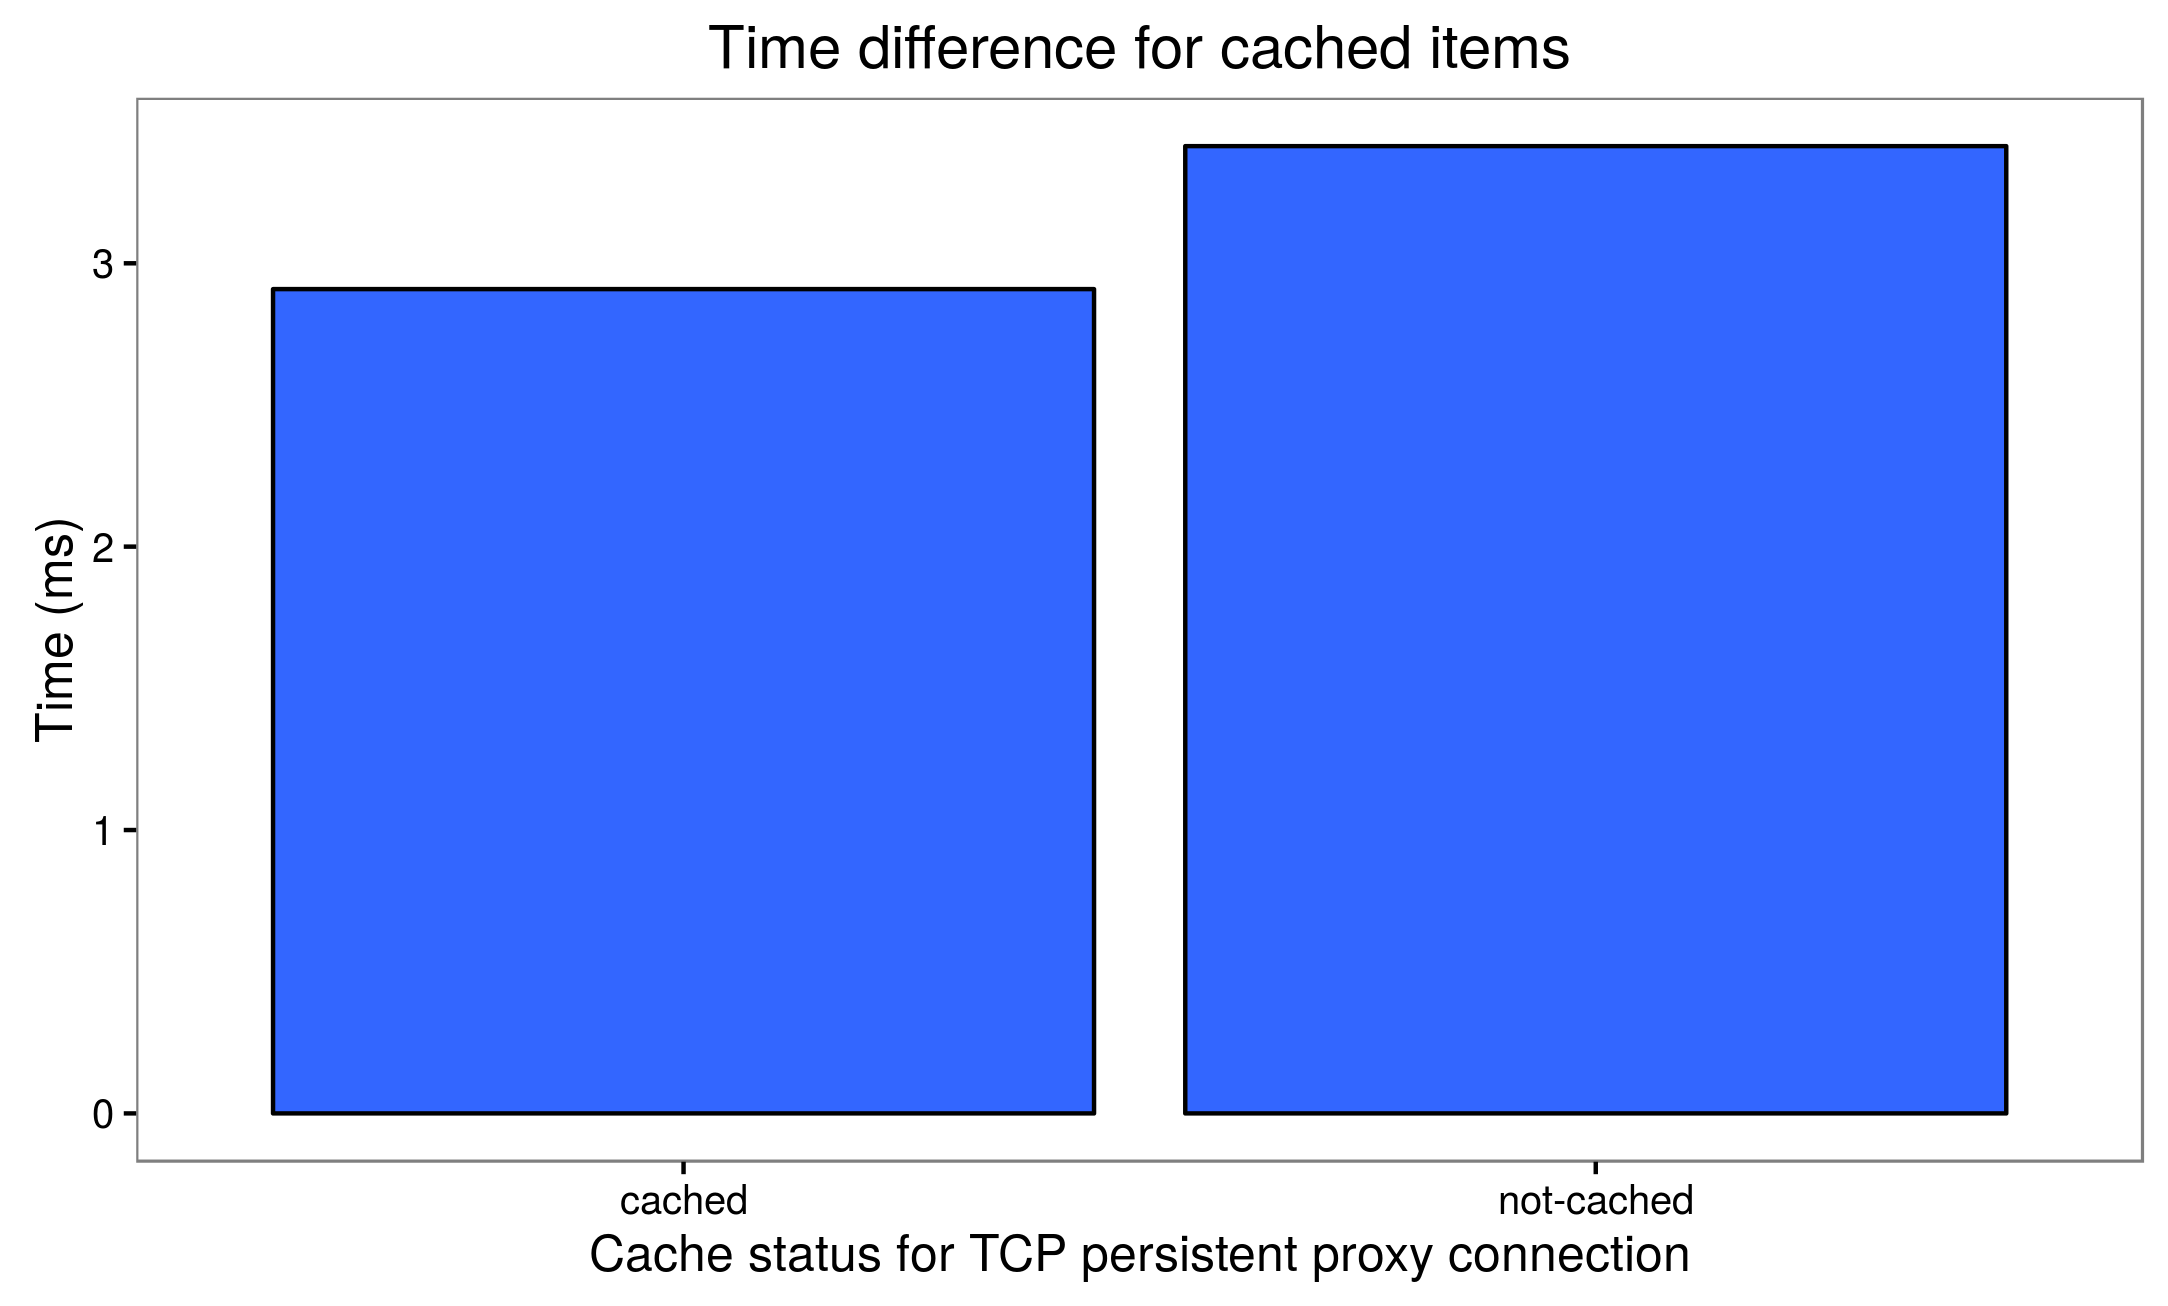
\includegraphics[width=\columnwidth]{resources/RTT_cache.png}
			\caption{RTT times for different cache statuses on a TCP persistent connection}
			\label{fig:rtt_cache}
		\end{figure}


	% subsubsection basic_client_server_http_requests_and_responses (end)
%%%%%%%%%%%%%%%%%%%%%%%%%%%%%%%%%%%%%%%%%%%%%%%%%%%%
\section{CRITICAL ANALYSIS}
		
		The system is a fully functional, stable and well constructed solution. The presented system implements all functionality stipulated in project brief, that being the following: web server, web client, proxy server, multithreading, persistent and non-persistent connection types, TCP and UDP, the use of Wireshark to obtained results and the use of a timer to obtain RTT values for different connection types. \\

		Despite the solution being fully functional there are three weaknesses. Firstly, the primary weakness of the system is that once the client establishes a connection with the proxy, all future computation (i.e. proxy communication with the server) until the response reaches the client takes place in a thread established by the proxy. Despite Go multithreading being able to handle thousands of threads at the same time with very little computational overhead, this is not the ideal implementation if the infrastructure utilising the proxy were to be on the level of a large scale business. Secondly, another design constraint was accepted when it was decided to only implemented TCP communication when the client was communicating with the server via the proxy. This was primarily due to the above mentioned problem. \\
		
		Thirdly, another minor weakness, which was primarily due to time constraints, was the inability to interact with web forms. This is due to the fact that JavaScript is often implemented in order to auto-generate the correctly structured POST message for the form. As a result of this a well rounded implementation of this could not be presented and a design decision was taken to omit this aspect. Despite this, the POST method still works when generating a basic example between the client and server.  \\
		
		There are multiple aspect of the system that are subject to improvements. Initially, creating a smart way of mapping client and sever IP addresses on the proxy will allow for the above mentioned thread problem to be fixed. This would be the primary priority of the project. Also, allowing the proxy to implement UDP communication would better the functionality range of the system. The other aspect of improvement would be increasing the overall scope of the project. Expansions to the system could be in the form of adding support for https and not only http and increasing the range of requests and responses to all those mentioned in Tables~\ref{httpreqs} and \ref{httpresps}.
	
	\subsection{Opportunities}
	
		


%%%%%%%%%%%%%%%%%%%%%%%%%%%%%%%%%%%%%%%%%%%%%%%%%%%%
\section{DESCRIPTION OF CODE}

	\subsection{Overall Code Structure}

		The project was structured such that all code was localised to a common root directory called \texttt{src/}. By localising the code in a source root directory it allowed for the client, server and proxy associated code to be located in this folder under their own subdirectories (i.e. \texttt{src/client/}). Due to this specific project layout a feature of Go is that all common functionality between the client, server and proxy code can be abstracted to a further subdirectory \texttt{src/lib/}, thus creating a library of common functionality for the project. This library can be sourced in any project script allowing that script access to all common functionality.\\
		
		The majority of the code was centralised around the functionality of structs. The main reason for doing this was to provide each struct with its own methods, a feature of the Go programming language. An example of this implementation can be seen in the listings excerpt from the \texttt{request\_message.go} file (Listings~\ref{lst:struct}). 
		
		\lstinputlisting[language=go, caption=Struct method setup, label={lst:struct}, style=go, breaklines=true, firstline=5, lastline=17]{../../src/lib/request_message.go}
		
		The function seen in Listings~\ref{lst:struct} can be invoked on a \texttt{RequestMessage} object, \texttt{rm}, by calling \texttt{rm.RequestMessage (arg1, arg2, arg3)} on the object. This proved beneficial when dealing with multiple objects of the same type as the information was localised to each struct object. \\
		
	\subsection{Configuration Settings}
		
		As there are multiple options available for the types of protocols, connections and proxy it was necessary to provide the user with the ability to change these settings in a "user friendly" manor. The configurations were set-up in a struct as this allowed for easy manipulation of the values as well as being able to implement read and write methods on a configuration file easily. The struct was defined as seen is Listing~\ref{lst:config_struct} of Appendix~\ref{app:config} while the code used to edit the configuration settings can be seen in Listing~\ref{lst:config_edit} of Appendix~\ref{app:config}. 
		
		
	\subsection{Client Code}
		
		The client code was mainly centralised around establishing a connection with either the web server or the proxy server. Once this connection was established it needed to ensure that all information was read from the server before analysing the received information. Upon analysis of this information, the client could be required to establish further connections to retrieve images and other sources before saving the file to a temporary directory to be launched. \\
		
		\subsubsection*{Establishing The Connection:} The type of connection that is established by the client is dependant on what protocol configuration setting was specified by the client. Despite this the \texttt{net} package in Go is able to accept either TCP or UDP when creating a network connection \cite{net}. The connection was established as can be seen in Listing~\ref{lst:client_conn} of Appendix~\ref{app:client}. 
		
		\subsubsection*{Retrieving Information:} In order to determine whether or not all the information had been obtained from the server it was required that initially the client would read a large packet from the connection. In this packet the client code would search for either the presence of either the header line \texttt{Transfer-Encoding:Chunked} or \texttt{Content-Length:\textit{<bytes>}}. The presence of either of these two header lines meant that the server had divided the sent file into multiple packets. The fact that all the headers are parsed into a map of header name to details it makes the look up fast and effective. \\
		
		In order to read multiple packets it was necessary to continuously loop over the read function until all the information had been obtained. Determining when to exit this loop was aided by the above mentioned header lines. Firstly the \texttt{Transfer-Encoding} is a header line specific to HTTP/1.1 which ensures that an End-Of-File character, \texttt{\textbackslash r\textbackslash n0\textbackslash r\textbackslash n\textbackslash r\textbackslash n}, will appear in the last packet. Therefore, searching each packet for this character provided the required knowledge. Secondly, the \texttt{Content-Length} provided knowledge of the size of the attached body. Therefore, utilising this and being able to manually calculate the size of the header lines meant that the packets could be read from the connection and continually subtracted from the running tally of remaining bytes until such time that the running tally became negative. The implementation of these two concepts can be seen in Listing~\ref{lst:client_read} of Appendix~\ref{app:client}. 
		
		\subsubsection*{Analysing Received Information:} The next important aspect of the client was determining whether or not the received file contained any references to other files that were imperative to the received file forming correctly. It was assumed that all references to other files would begin with "src=http://" in the base HTML file, all other file references were ignored as they would be beyond the scope of the project.\\
		
		String manipulation was used to determine the presence of these sources. If there were any sources present the \texttt{retrieveSources()} function, see Listing~\ref{lst:client_ret} of Appendix~\ref{app:client}, would deconstruct the referenced strings through the use of regular expressions and the occurrence of special characters. From the deconstruction the function constructs a map of host name to file extension on the hosts server. The map would then be used to iterate over all elements in the map and retrieve them as described in the above sections.
				
	\subsection{Server Code}
	
		As in the case of the client code the server code was primarily revolved around certain concepts. These concepts are: confirming and establishing the connection with the client, processing the clients request, generating the appropriate response to the client's request and sending the generated information to the client. The server has additional functionality in two aspects, namely: when interfacing with the proxy it has to determine if a cached file has been recently updated and when interfacing with the client it has to prove the new location of a page if it has been moved.  
		
		\subsubsection*{Listening For and Establishing a Connection:} Unlike the case for the client, the server side calls for the implementation of TCP and UDP differ. Thus, in order to account for this, two separate functions were implemented to establish the individual connections. The code used to implement these connection can be seen in Listing~\ref{lst:server_conn} of Appendix~\ref{app:server}. Two aspects of Listing~\ref{lst:server_conn} need to be noted. Firstly, the listening function calls differ (lines 20 and 40) and secondly in lines 5 and 6 there is the implementation of the \texttt{go <function>} command which is the Go programming language implementation of establishing a new thread. Therefore, each time a new connection request is received by the server, the request is handled in a new thread. 
		
		\subsubsection*{Processing The Client Request:} Processing the client request requires decomposing the client request message to obtain the HTTP method, the required URL, the HTTP version being used by the client, the header field lines and the body (if one is attached). Depending on this information the server is able to perform certain conditional checks in order to generate the correct response message. 
		
		\subsubsection*{Taking Action and Generating Response Message:} The HTTP method will determine the course of action that the server follows, these are detailed in Table~\ref{httpreqs}. The method of interest is the GET method. The GET method firstly requires the server to check if the file exists and secondly, if it does exist, to retrieve a copy of the file and parse it into the response message to be sent to the client. If the file does not exist or there was another problem with the client request message, the server would generate the appropriate error message detailed in Table~\ref{httpresps}.
		
		\subsubsection*{Server Proxy Interfacing:} The proxy interaction will make specific reference to the GET request as this encompasses all functionality. The implementation of the GET response code can be seen in Listing~\ref{lst:server_prox} of Appendix~\ref{app:server}. \\
		
		If the proxy contains a copy of the requested file it appends a \texttt{Last-Modified} header line to the request message, this is what the server looks for. If there is a date mentioned the server then compares if the file has been modified since that date (the last modified date can be obtained from the function call in line 7 of the listing), this is achieved through the use of the \texttt{time.After()} function in the \texttt{time} Go package (see line 11 of the listing). If the file has been modified then the server returns the latest copy of the file and if it hasn't it returns the \texttt{304 Not Modified} response. \\
		
		\subsubsection*{Moved Files:} In order to determine whether or not a file has been moved the server keeps a table of file previous location and current location for all moved files, this is stored as a text file on the server. When a request for a file is made, if the location appears in this file the server composes a \texttt{301} response message and appends a \texttt{Location} header with the new location to the header field.
		
	\subsection{Proxy}
		
		The proxy sending and receiving of information is identical in nature to the corresponding implementations in the client and server, therefore the only aspect of the proxy that will be analysed is caching. Two characteristics of proxy caching is the storing of files and the conditional gets. \\
		
		\subsubsection*{File Storing:} File storing is only implemented for GET requests. When the response message is received from the server the proxy creates a directory in the cache corresponding to the full path of the file received from the server. A design decision was taken to "mimic" the server in the proxy as opposed to mapping file names to a different location in the cache. The code used to create a directory with full read write permission can be seen in line 3 of Listing~\ref{lst:proxy_cache} of Appendix~\ref{app:proxy}. Once the directory is created the code then writes the corresponding file to the location, this can be seen in line 6 of the listing.
		
		\subsubsection*{Conditional Get:} The conditional GET revolves primarily around the aforementioned \texttt{304} response code from the server. When the proxy receives the clients request message it checks if the file occurs in the proxy cache, see line 1 of Listing~\ref{lst:proxy_cond}. This is achieved by using the look-up table stored on the proxy of URL to last-modified times. If the file does occur in cache the client request message is modified by including the last-modified date in the look-up table. This is simple to do as the headers are stored as a map already. The proxy then obtains the response message from the server which either specifies that the file was modified or it was not. \\
		
		If the file is not modified then the proxy retrieves the file from cache and forwards a copy of it to the client. If the file has been modified then new file is written to cache as mentioned above and the cache map is modified to contain the new date, this implementation can be seen in lines 12-16 of Listing~\ref{lst:proxy_cond}. 
	
	\subsection{All Other Common Functionality}
	
		The above mentioned sections were described in detail as they are fundamental to the functionality of the system. The other common functions implemented in the project are described in brief in Table~\ref{tab:functions} of Appendix~\ref{app:other_func}.

%%%%%%%%%%%%%%%%%%%%%%%%%%%%%%%%%%%%%%%%%%%%%%%%%%%

\section{CONCLUSION}

%%%%%%%%%%%%%%%%%%%%%%%%%%%%%%%%%%%%%%%%%%%%%%%%%%%

\begin{thebibliography}{1}

\bibitem{kurose} Kurose J F, Ross K W. \emph{Computer networking: a top-down approach.} Boston, Pearson. 2013. pp 83 - 115.

\bibitem{rfc7230} Fielding R, Reschke J. `Hypertext Transfer Protocol (HTTP/1.1): Message Syntax and Routing.' IETF, RFC June 2014. [online] Available: \url{https://tools.ietf.org/html/rfc7230}

\bibitem{rfc1945} Berners-Lee T, Fielding R, Frystyk H. `Hypertext Transfer Protocol -- HTTP/1.0' IETF, RFC May 1996. [online] Available: \url{https://tools.ietf.org/html/rfc1945}

\bibitem{guinard}   Guinard D, Trifa V (2009). \emph{Towards the Web of Things: Web Mashups for Embedded Devices.} Workshop on Mashups, Enterprise Mashups and Lightweight Composition on the Web (MEM 2009), in proceedings of WWW (International World Wide Web Conferences). Madrid, Spain. April 2009.  

\bibitem{doxsey} Doxsey C. \emph{An Introduction to Programming in Go.} 2012. ch 10. pp 108 - 111.

\bibitem{net} The Go Programming Language. \emph{Package net.} The Go Programming Language. Available: \url{https://golang.org/pkg/net/#Dial}.


\end{thebibliography}

%%%%%%%%%%%%%%%%%%%%%%%%%%%%%%%%%%%%%%%%%%%%%%%%%%%
\onecolumn
\clearpage
\newpage
\appendix
\section{Results supporting information} % (fold)
\label{sec:results}
	
	This appendix details the results obtained when running the application one two separate computers on the same network. The results include excerpts of the results obtained from Wireshark as well as the Round Trip Times (RTT) obtained for different implementations of the project.

	\subsection{Wireshark results} % (fold)
	\label{sub:wireshark_results}
	
		\begin{figure}[h!]
			\centering
			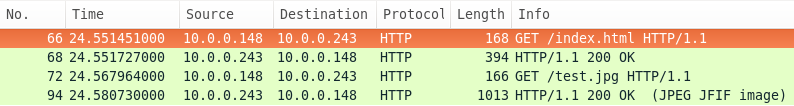
\includegraphics[width=\columnwidth]{resources/get_html}
			\caption{Computer interaction for GET request}
			\label{fig:basic_get}
		\end{figure}
		
		\begin{figure}[h!]
			\centering
			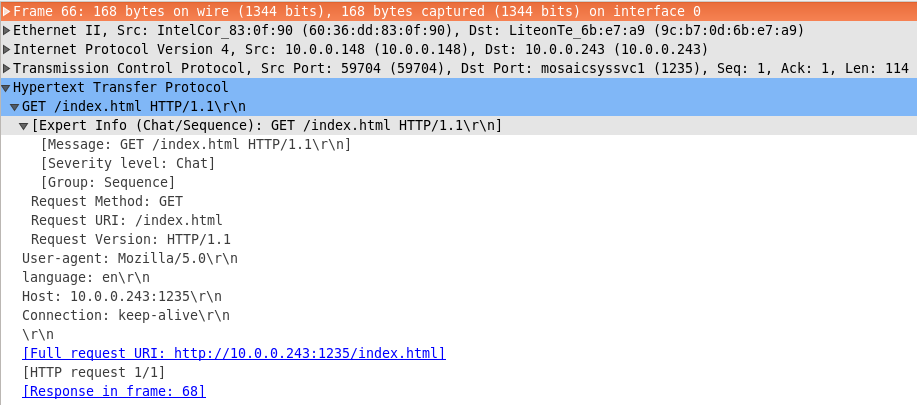
\includegraphics[width=\columnwidth]{resources/message_get_html}
			\caption{GET request message}
			\label{fig:basic_get_message}
		\end{figure}
		
		\begin{figure}[h!]
			\centering
			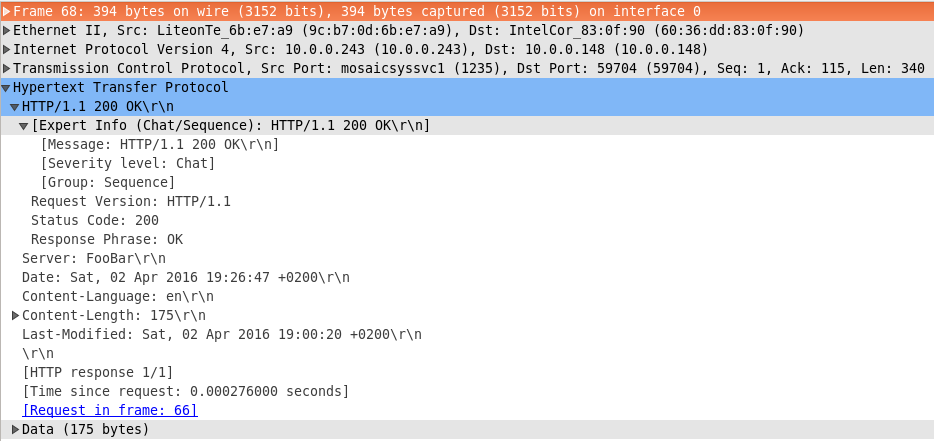
\includegraphics[width=\columnwidth]{resources/message_get_response_html}
			\caption{GET response message}
			\label{fig:basic_get_response}
		\end{figure}
		
		\begin{figure}[h!]
			\centering
			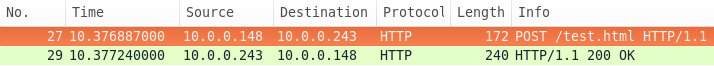
\includegraphics[width=\columnwidth]{resources/post_request}
			\caption{POST trace between client and server}
			\label{fig:basic_post}
		\end{figure}
		
		\begin{figure}[h!]
			\centering
			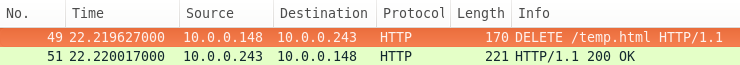
\includegraphics[width=\columnwidth]{resources/delete_request}
			\caption{DELETE trace between client and server}
			\label{fig:basic_delete}
		\end{figure}
		
		\begin{figure}[h!]
			\centering
			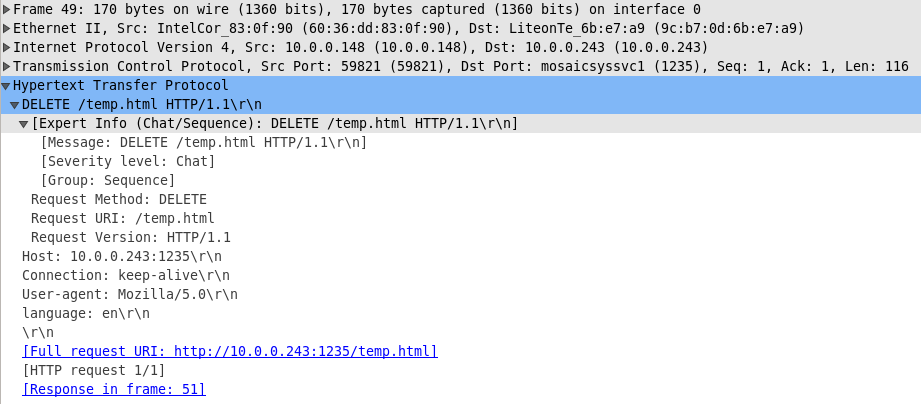
\includegraphics[width=\columnwidth]{resources/delete_request_message}
			\caption{DELETE request message}
			\label{fig:basic_delete_message}
		\end{figure}
		
		\begin{figure}[h!]
			\centering
			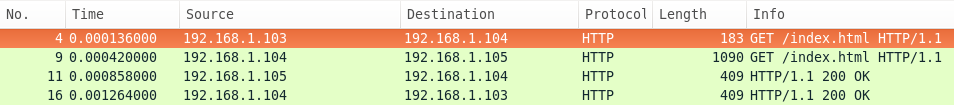
\includegraphics[width=\columnwidth]{resources/proxy_new}
			\caption{GET request for proxy with no cache saved}
			\label{fig:proxy_new}
		\end{figure}
		
		\begin{figure}[h!]
			\centering
			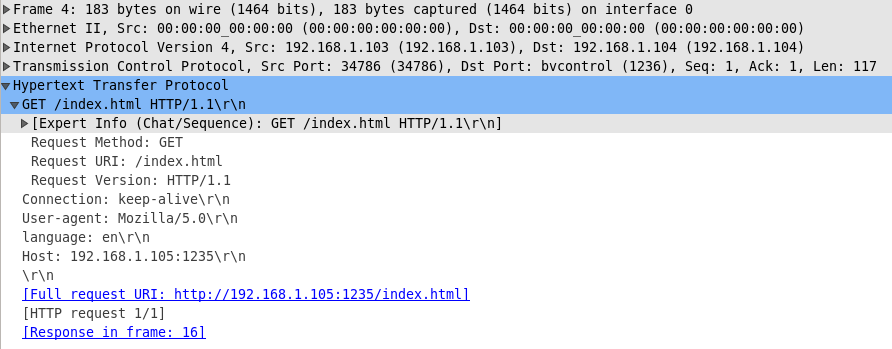
\includegraphics[width=\columnwidth]{resources/proxy_new_client}
			\caption{GET request message for client to proxy with no cache saved}
			\label{fig:proxy_new_client}
		\end{figure}
		
		\begin{figure}[h!]
			\centering
			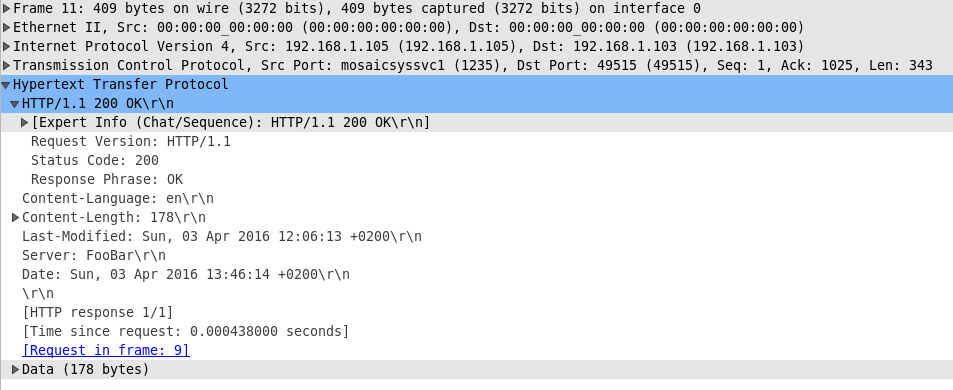
\includegraphics[width=\columnwidth]{resources/proxy_server}
			\caption{GET response message from server to proxy}
			\label{fig:proxy_server}
		\end{figure}
		
		\begin{figure}[h!]
			\centering
			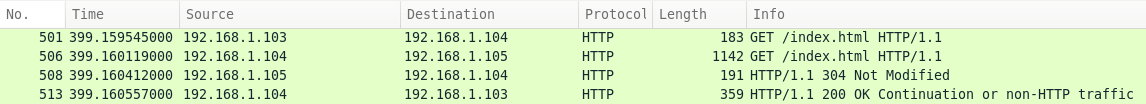
\includegraphics[width=\columnwidth]{resources/proxy_cache}
			\caption{GET request message for client to proxy with saved cache}
			\label{fig:proxy_cache}
		\end{figure}
		
		\begin{figure}[h!]
			\centering
			\subfloat[Proxy GET before caching]{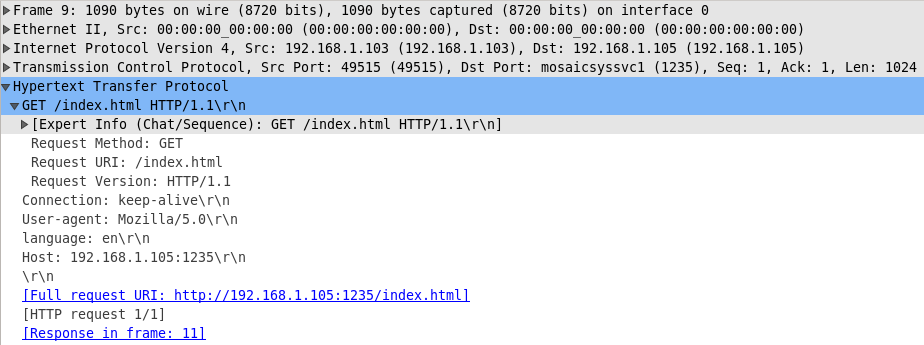
\includegraphics[width = 0.46\columnwidth]{resources/proxy_new_get}} \hspace{1cm}
			\subfloat[Proxy GET after caching]{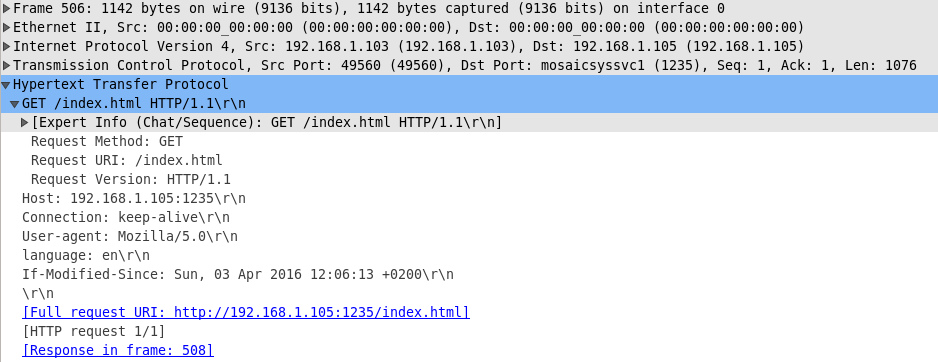
\includegraphics[width = 0.46\columnwidth]{resources/proxy_get_cache}}
			\caption{Difference in proxy request messages depending on status of cache}
			\label{fig:proxy_comparrison}
		\end{figure}
		
	\subsection{RTT Results}
	\label{app:rtt}
		
		\begin{figure}[h!]
			\centering
			\subfloat[301]{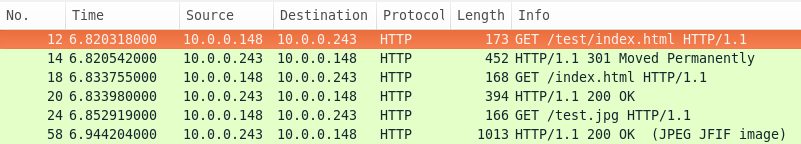
\includegraphics[width =\columnwidth]{resources/301}} \\
			\subfloat[400]{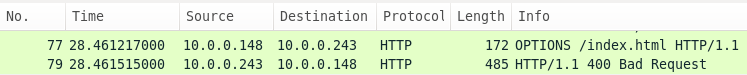
\includegraphics[width = \columnwidth]{resources/400}} \\
			\subfloat[404]{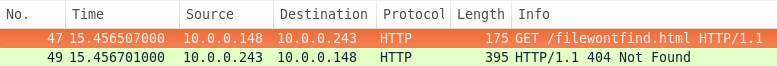
\includegraphics[width = \columnwidth]{resources/404}} \\
			\subfloat[505]{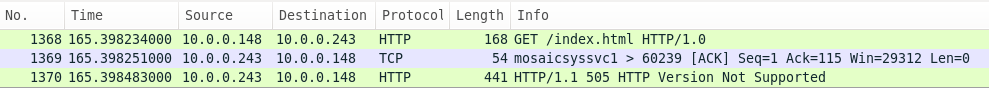
\includegraphics[width = \columnwidth]{resources/505}} \\
			\caption{Different server error response codes}
			\label{fig:server_error}
		\end{figure}
		
		\begin{figure}[h!]
			\centering
			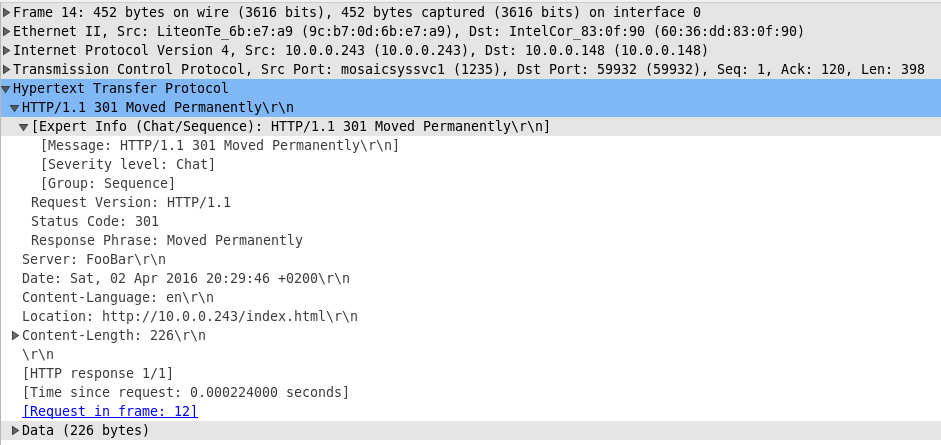
\includegraphics[width=\columnwidth]{resources/301_response_message}
			\caption{301 Server response message with location header field}
			\label{fig:301}
		\end{figure}
\clearpage
\section{Code Description Supporting Information}
	
	This appendix serves to provide additional information for the detailed analysis of the code implemented in the project.
	
	\subsection{Configuration Settings}
	\label{app:config}
		
		\lstinputlisting[language=go, caption=Struct for configuration settings, label={lst:config_struct}, style=go, breaklines=true, firstline=10, lastline=14]{../../src/lib/config_settings.go}
		
		\lstinputlisting[language=go, caption=Manipulation of configuratuion settings, label={lst:config_edit}, style=go, breaklines=true, firstline=36, lastline=62]{../../src/lib/config_settings.go}
		
	\subsection{Client}
	\label{app:client}
	
		\lstinputlisting[language=go, caption=Establishing client sever initial connection, label={lst:client_conn}, style=go, breaklines=true, firstline=66, lastline=68]{../../src/client/client.go}
		
		\lstinputlisting[language=go, caption=Client read from connection, label={lst:client_read}, style=go, breaklines=true, firstline=113, lastline=148]{../../src/client/client.go}
		
		\lstinputlisting[language=go, caption=Client retrieve sources function, label={lst:client_ret}, style=go, breaklines=true, firstline=247, lastline=266]{../../src/client/client.go}
		
	\subsection{Server}
	\label{app:server}
	
		\lstinputlisting[language=go, caption=Server TCP and DUP handing, label={lst:server_conn}, style=go, breaklines=true, firstline=19, lastline=65]{../../src/server/server.go}

		\lstinputlisting[language=go, caption=Server proxy GET interfaction, label={lst:server_prox}, style=go, breaklines=true, firstline=186, lastline=225]{../../src/server/server.go}
		
	\subsection{Proxy}
	\label{app:proxy}
	
		\lstinputlisting[language=go, caption=Server proxy GET interfaction, label={lst:proxy_cache}, style=go, breaklines=true, firstline=116, lastline=121]{../../src/proxy/proxy.go}
		
		\lstinputlisting[language=go, caption=Conditional GET, label={lst:proxy_cond}, style=go, breaklines=true, firstline=59, lastline=77]{../../src/proxy/proxy.go}
		
	\subsection{Other Functionality}
	\label{app:other_func}
		\begin{table}[htbp]
			\centering
			\scriptsize
			\caption{Different methods for invoking server response errors}
			\label{tab:functions}
			\begin{tabular}{p{0.2\columnwidth}| p{0.2\columnwidth} | p{0.1\columnwidth} | p{0.45\columnwidth}}
				\hline
				\textbf{Function Name} & \textbf{File} & \textbf{Author} & \textbf{Description} \\ \hline
				newRoundTripTimer & timer.go & DT & Create new timer struct object \\
				loadTimerMap & timer.go & DT & Load pre-existing timer values \\
				startTimer & timer.go & DT & Start the timer \\
				stopTimer & timer.go & DT & Stop the timer and calculate duration \\
				addToTimer & timer.go & DT & Add the new values to the timer map \\
				writeTimerToFile & timer.go & DT & Write new timer values to the timer map file \\
				CheckError & check\_error.go & JA & Interpret system error \\
				ReadConfig & config\_settings.go & DT & Read configuration settings from file \\
				InitializeConfig & config\_settings.go & DT & Initialize the configuration settings to last known settings \\
				WriteConfig & config\_settings.go & DT & Write configuration settings to configuration file \\
				CheckInput & config\_settings.go & DT & Interpret the user input for changing a specified configuration \\
				DecomposeRequest & decompose\_request.go & JA & Extract the HTTP method, desired URL, HTTP version, header lines, and body from the client request message \\
				DecomposeResponse & decompose\_response.go & DT & Extract the HTTP version, status code, status message, header lines, and body from the server response message \\
				FileExists & file\_exists.go & JA & Determine if the file at the desired path exists \\
				NewRequestMessage & request\_message.go & DT & Create new request message struct object \\
				SetRequestLine & request\_message.go & DT & Set the request line of the request message object \\
				SetHeaders & request\_message.go & DT & Set the header lines of the request message object \\
				SetEntityBody & request\_message.go & DT & Set the entity body of the request message object \\
				SetRequestMessage & request\_message.go & DT & Call the above three set methods on the request message object \\
				ToString & request\_message.go & DT & Convert the request message object into a string \\
				ToBytes & request\_message.go & DT & Convert the request message string into bytes \\
				NewReponseMessage & response\_message.go & JA & Create a new response message struct object \\
				ToString & response\_message.go & JA & Convert the response message object to a string \\
				ToBytes & response\_message.go & JA & Convert response message string to bytes \\
				loadMap & map\_handler.go & DT & Load text file from server into a map \\
				saveMap & map\_handler.go & DT & Save new map to the server as a text file \\
				handleRequest & client.go &	DT & Responsible for handling the request to the server dependant on configuration settings \\
				writeReceivedToFile & client.go & DT &	Write the received file from the server to a temporary file for launching \\
				getRedirectionLocation & client.go &	DT & If the server response is a 301/302 then determine the new location of the file from the response message \\
				getUserInputs & client.go &	DT & Get the user to input the HTTP method, URL and body if the method was PUT or POST \\
				getFileName & client.go &	DT & Retrieve the file name from the entire URL string \\
				retrieveSources & client.go &	DT & Extract all the sources from the body of the response message and place them in a map \\
				printToConsole & client.go &	DT & Print the server response message to console \\
				getHeaderSize & client.go &	DT & Get the size of the response message headers in bytes \\
				startTCPServer & server.go & JA & Establish a TCP connection with the client \\
				startUDPServer & server.go & JA & Establish a UDP connection with the client \\
				handleUDPClient & server.go & JA & 	Perform read and write functionality for UDP client \\
				handleTCPClient & server.go & JA & Perform read and write functionality for TCP client \\
				composeResponse & server.go & JA & Compose a new server response message based on the HTTP method and URL supplied by the client request message \\
				loadMovesMap & server.go & JA & Load The map containing the previous and current location of all objects that have been moved \\
				handleClient & proxy.go & JA & Handle all read and write functionality for proxy-client interface \\
				getNewResponse & proxy.go & JA \& DT & Compose a new response message depending of the status of the cache \\
				checkInCache & proxy.go & JA & Checking if the file exists in the proxy cache \\
				modifyHeaders & proxy.go & DT & Modify the headers based on last modified information from cache \\
				compileNewRequest & proxy.go & DT & Compile a new request message \\
				handleServer & proxy.go & DT & Handle all read and write functionality for proxy-server interface \\
				getHeaderSize & proxy.go & JA & Get the size of the message header field \\				
				\hline
			\end{tabular}
		\end{table}

\clearpage
\section{Time Management}
\label{app:time_man}
	\begin{figure}[h!]
		\centering
		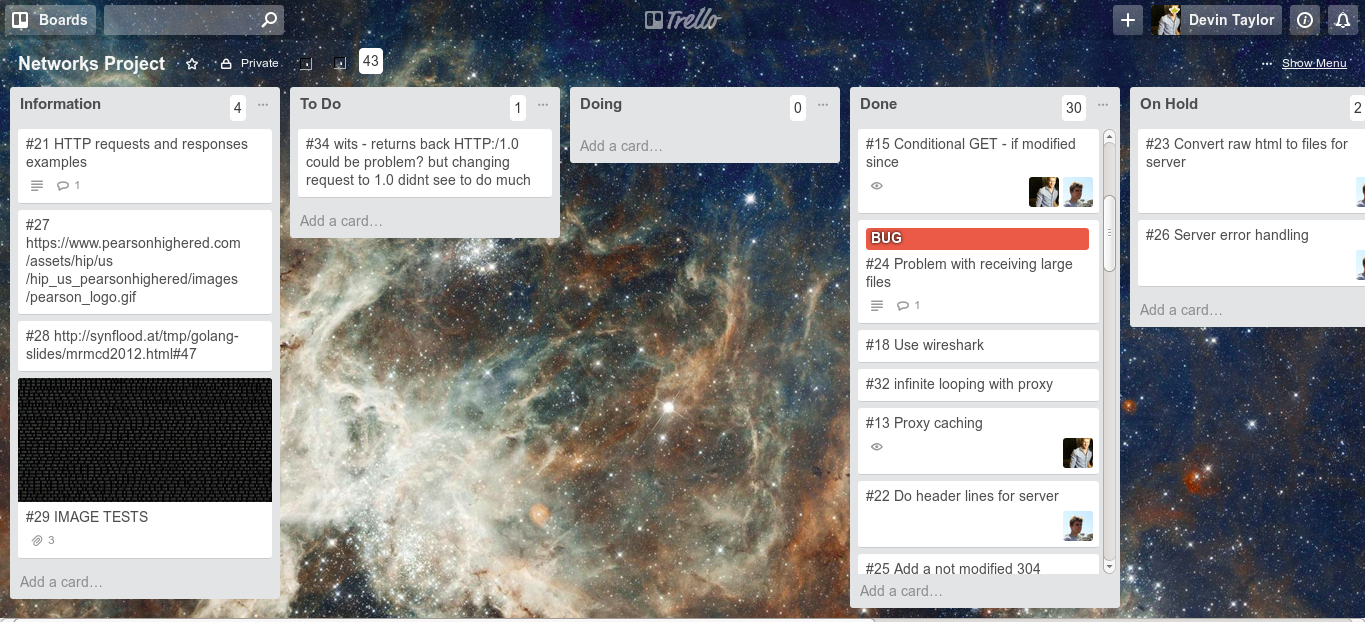
\includegraphics[width=\columnwidth]{resources/trello_networks}
		\caption{Screen shot of Trello board used}
		\label{fig:trello}
	\end{figure}
	
	\begin{figure}[h!]
		\centering
		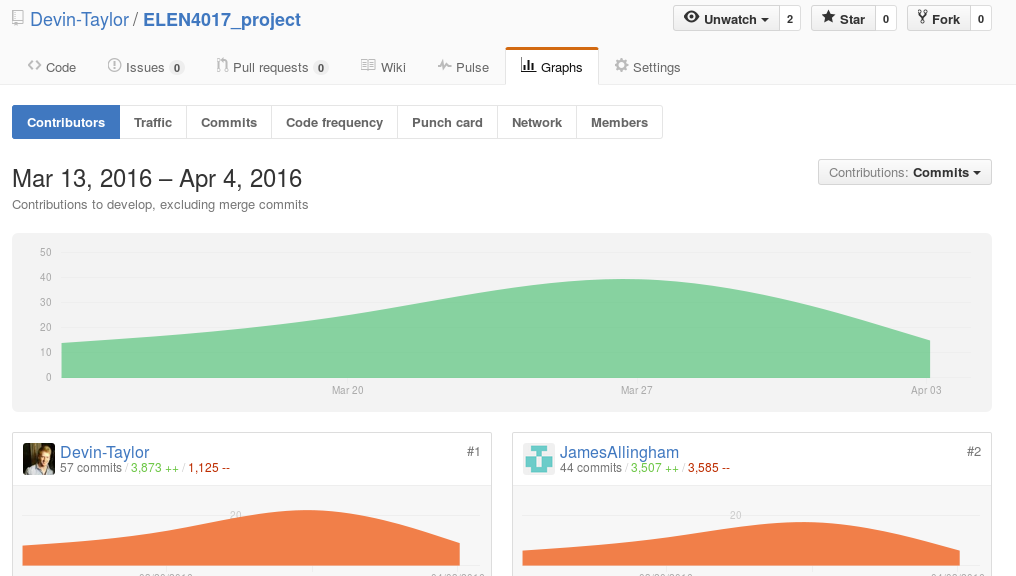
\includegraphics[width=\columnwidth]{resources/github_code}
		\caption{Screen shot of GitHub contributions}
		\label{fig:github}
	\end{figure}
	
% section results (end)

\end{document}